\chapter{System Analysis}
\section{Introduction}
After we collected a lot of information about our users and competitors,In this chapter we provide detailed information about our system including functional requirements, non-functional requirements, user requirements, system architecture, use case, and sequencing diagrams.
\section{System Requirements}
Requirements are not about the solution ideas, but it is about what are the needs of the user and the ability of our project to implement these requirements.System requirements are the needed configurations for the system to operate efficiently.The next three subsections will discuss the functional requirements,Nonfunctional requirements, and user requirements.
\subsection{Functional Requirements }
In systems engineering, functional requirements are directly related to system services. Functional software requirements help you capture files of the system's intended behavior. This behavior can be expressed as functions, services, tasks, or any system required to perform. In this subsection, we list the functions that are required in our system.
\subsubsection{Permits the user to scan affected area}
The system provides a way to scan skin affected area through mobile application.
\subsubsection{Shows the matched results after processing}
Using deep learning, the system shows top matched results with the scanned photo.  
\subsubsection{Explains how to deal with symptoms on the body}
After scan report, the system explains to the user more details about his case in a simple way to understand.
\subsubsection{Ordering medicines and Asking a doctor}
Provides the ability to order medicines and book an appointment with the dermatologist.
\subsubsection{Providing a database of more than 620 types of skin diseases}
The user can search for a disease by name and get the disease information, Self-care, Medicines that can be used, Additional information (causes and places of spread) and any other disease with the same symptoms.
\subsection{Non Functional Requirements}
The system needs to operate efficiently and meet the requirements. Any failure of the components of the systems may lead to one or more of functions to stop or be misused. A non-functional requirement is a requirement that specifies criteria that can be used to judge the operation of a system.
\subsubsection{Accessibility}Easy design that is suited for different communities to use.
\subsubsection{Availability}Available for low versions of android devices as well as high versions.
\subsubsection{Capacity	}Low storage space consumption.
\subsubsection{Minimize response time (high speed)}System response within few seconds.
\subsubsection{Performance}High (recognition and detection) tools and algorithms.
\subsubsection{Reliability and Safety	}System should be safe so patient can rely on.
\subsubsection{Usability}Easy to use and understand for different users.
\subsubsection{Security}Only user ( patient) can allow the system to keep and capture their diagnostic image and use it in the training process and make adjustments to their data.
\subsection{Design Objectives }
Without doubt, one of the most important objectives of this phase is to build an accessible, usable and engaging digital product that fills our users' needs.
\newpage
\subsection{User Requirements}
The user of the application is a patient who wants to know the result of his medical test by capturing or upload a photo of an affected area with unknown symptoms on his body.
\vspace{0.50cm}
\begin{enumerate}[label=\fbox{\arabic*}]
	\item Log in to the system.
	\item Scan affected area or upload a photo.
    \item Answer some questions about the case.
    \item Get the top matched results.
    \item Select the most appropriate diagnosis for your case.
    \item Get an explanation contains Self-care, Medicines that can be used, Additional information (causes and places of spread) and any other disease with the same symptoms.
    \item Get the medicines
    \item Book an appointment with the dermatologist.
    \item Search for a skin disease you want to know about.
    \item Contact technical support if there is a problem.
\end{enumerate}
\newpage
\section{System Architecture}
After determining the requirements of the system, we will describe its major 
Components, their relationships (structures), and how they interact with each
other.
\begin{figure}[!ht]
\centering
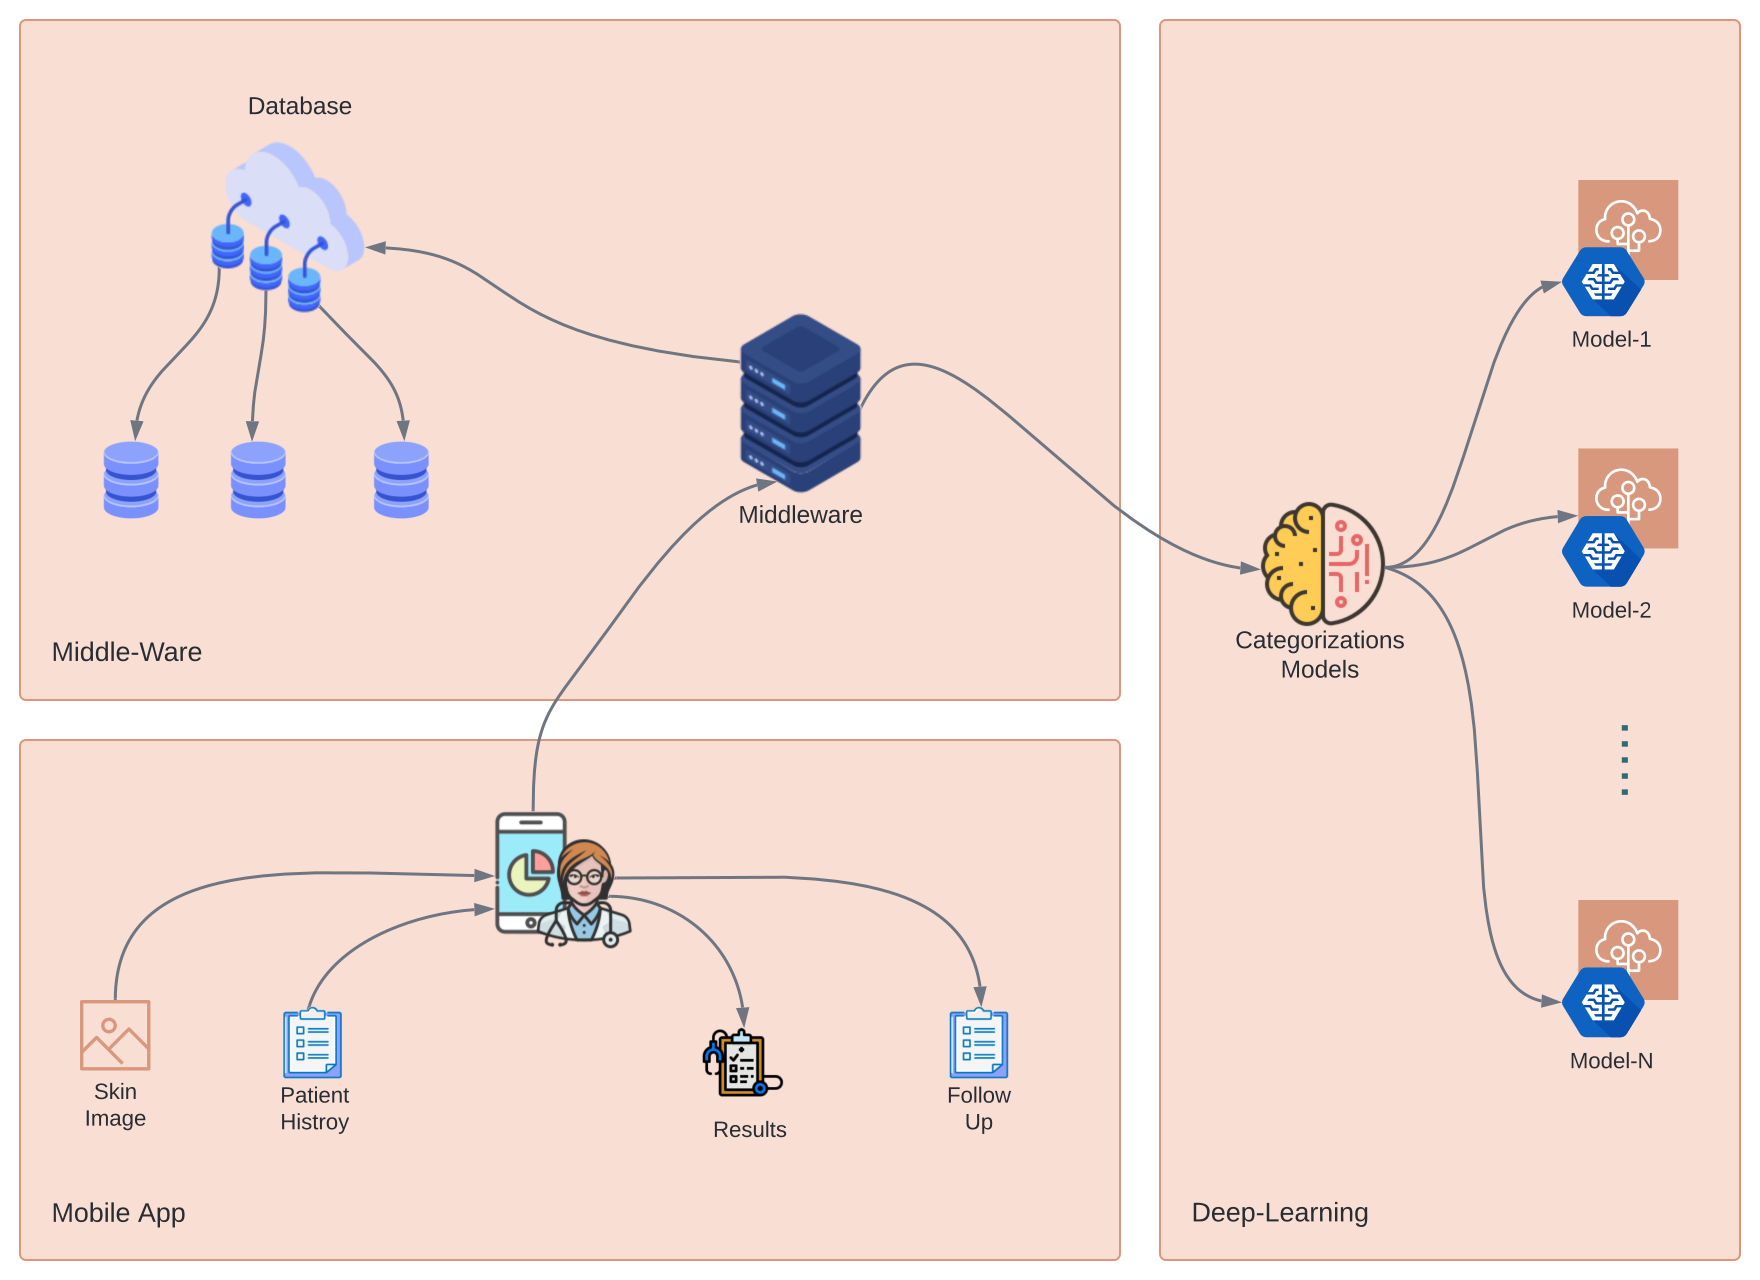
\includegraphics[width = 5.5in]{backmatter/figures/SysArch.png}
\end{figure}
\vspace{0.25cm}
\begin{itemize}
  \item \textbf{Mobile app subsystem:} user write about his medical history (if he didn’t sign in before ) and answer some questions about his situation and take image for disease or (upload from gallery) then app will replay with the prediction of disease and some information about it .\\Doctors will write information and medicines for diseases on the website and they will insert in database.\\
  \item \textbf{Middle-Ware subsystem:} Middle-Ware back-end will process information from doctors and users 
  beside information about users and doctors  and it will be responsible of 
  :\\
    \begin{itemize}
        \item Communicate with categorization models API to categorise disease from images and choice between them.\\
        \item Process answers of with storaged answers and information.\\
        \item Reply disease and information about it to user.\\
    \end{itemize}
  \item \textbf{Deep-Learning subsystem} microservices communicate with middle-ware to respond predictions of diseases.\\Microservices distributed between servires communicate with eath other.
\end{itemize}
\section{Development Methodology}
After we knew the basic structure of the system. We are going to view 
all of its functions, the relation between them  and the sequence of 
their executions in the following subparts.
\subsubsection{Use Case Diagrams}
First, with use case diagram, we will specify the expected behavior of the system. This helps us to 
design the system from end user's perspective.
\begin{figure}[!ht]
    \centering
    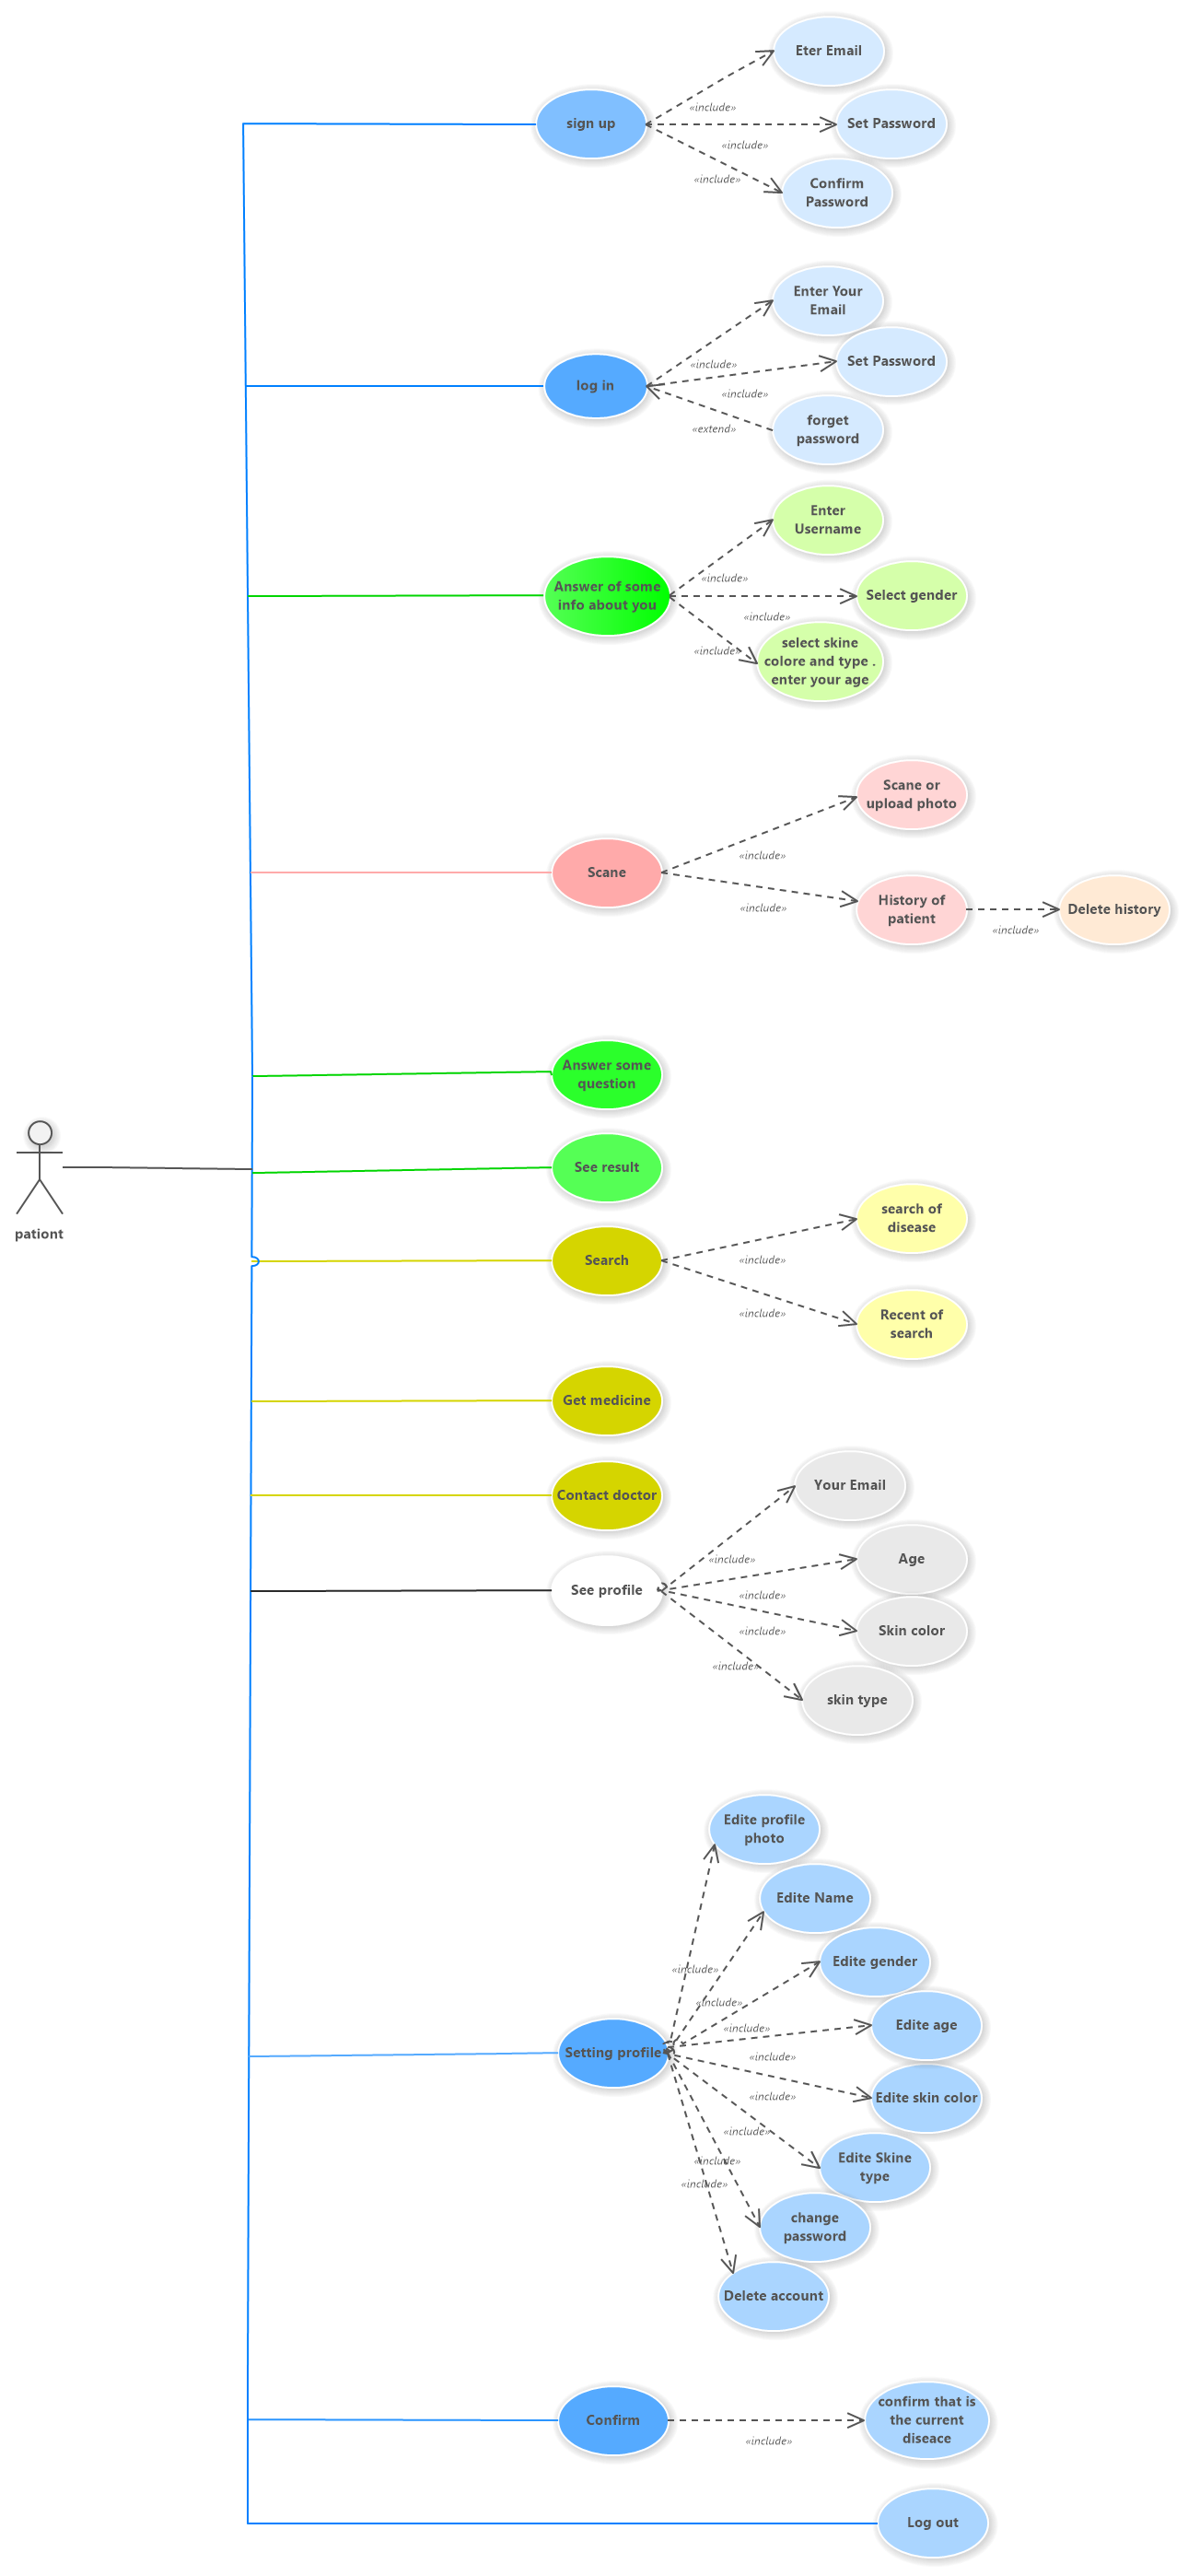
\includegraphics[width =8cm]{backmatter/figures/usecase.png}
    \caption{Use case diagram}
\end{figure}
\newpage
\subsubsection{Use Case Description }
\begin{itemize}
    \item \textbf{Use Case    :  DermAI}
    \item \textbf{Actors      :  Patient}
    \item \textbf{Goal        :  }The project aims to develop a healthcare system Uses artificial intelligence and machine learning techniques In diagnosing diseases starting with the largest organ in the body The human skin, which is the protective shield for the body The part that is most sensitive and vulnerable to environmental influences external.
     
    \item \textbf{Description :} When user scan his skin disease image , the 
    system analyzes it after 
    the user asks some questions about his disease and explains the result in 
    details. The system 
    suggests to the user the appropriate medicine , contact the nearest doctor 
    and he can search for any disease. He can also edit his profile.\\
\end{itemize}
\subsubsection{Sequence Diagram}
The sequence diagrams will show you how an operation is done and the inner 
details of it . To use our system, the user must be authorized first by sign up 
if it the first time or by login if he he owns an account. Once the user logged 
in successfully, his/her corresponding record in the database.
\begin{figure}
    \centering
    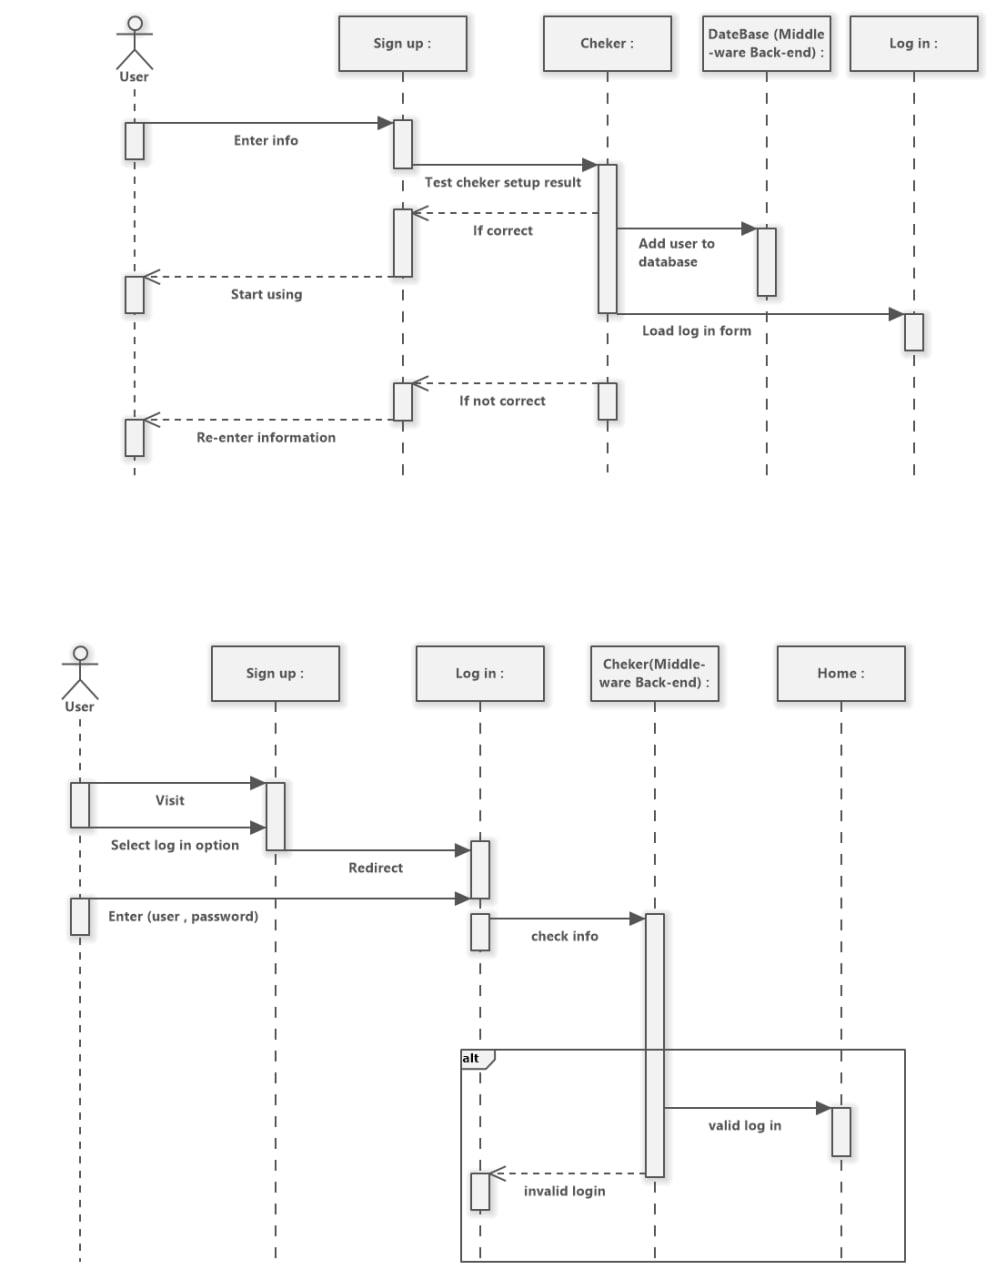
\includegraphics[width = 12cm]{backmatter/figures/Seq/loginlogout.jpg}
    \caption{login and log-out sequence diagram}
\end{figure}

\begin{figure}
	\centering
	\includegraphics[width = 12cm]{backmatter/figures/Seq/scan.jpg}
	\caption{scan images sequence diagram}
\end{figure}
\begin{figure}
	\centering
	\includegraphics[width = 12cm]{backmatter/figures/Seq/scanback.jpg}
	\caption{images processing in middle-ware sequence diagram}
\end{figure}
\begin{figure}
	\centering
	\includegraphics[width = 12cm]{backmatter/figures/Seq/search.jpg}
	\caption{search for diseases sequence diagram}
\end{figure}
\begin{figure}
	\centering
	\includegraphics[width = 12cm]{backmatter/figures/Seq/searchback.jpg}
	\caption{search for diseases processing in middle-ware sequence diagram}
\end{figure}

\newpage
\section{Tools and Languages}
Developing our software application can be divided into main two parts, which 
are the design part, the implementation part. \\\\
The design part involves designing diagrams and designing user interface of the
mobile application.\\\\
The implementation part involves programming languages, IDEs, frameworks, and 
libraries. The following list shows the needed tools for the software 
development and a brief description about their usages:\\
\begin{enumerate}
  \item \textbf{Software Ideas Modeler : }it is used to draw the UML diagrams.
  \item \textbf{Adobe XD : }it is used to design user interfaces and prototypes.
  \item \textbf{Android Studio : }it is an IDE to build mobile application for Android OS.
  \item \textbf{Postman : }it is an HTTP client that tests HTTP requests.
  \item \textbf{Visual Studio : }it is a set of development tools available in the form of visual studio add-in.
  \item \textbf{PhpMyAdmin : }Open source administration tool for MySQL and MariaDB. 
  \item \textbf{Skipper : }it is a visualization tool and code/schema generator for PHP ORM framework.
\end{enumerate}
\section{Summary}
 In this chapter we provide the reader with detailed knowledge about our system.Part 2 include system requirements Which is divided into functional , non-functional and user requirements which specify some different specifications for users. Part 3 includes system architecture which describe the main components of the system, their relationships, and how they interact with each other.Part 4 include development methodology which includes UML diagrams that shows the details of  how will the system work. In the end of the chapter we listed the needed tools to build the system.